\documentclass[12pt]{article}

\usepackage{scrtime} % for \thistime (this package MUST be listed first!)
\usepackage{fancyhdr}
\usepackage{xspace} %for having the perfect spacing after new commands
\usepackage{xcolor,colortbl}%for changing cell colour in tables
\usepackage{booktabs} %for tables
\usepackage{graphicx}
\usepackage{listings}
%\usepackage{Sweave}
%%%%formating the page%%%%
\pagestyle{fancy}

\usepackage{hyperref}
\hypersetup{colorlinks=true,linkcolor=blue,filecolor=magenta,urlcolor=cyan,}
\urlstyle{same}


\setlength{\headheight}{15.2pt}
\setlength{\headsep}{13 pt}
\setlength{\parindent}{28 pt}
\setlength{\parskip}{12 pt}
\pagestyle{fancyplain}
\usepackage[T1]{fontenc}
\rhead{\fancyplain{}{Genetic Distance and Pangenome Size Correlation $|$  \today \hfill Ann Le}} %insert your name here and your document title. the \today will just put the date that you compiled the documnet there.
\renewcommand\headrulewidth{0.5mm}
%%%%%%%%%%%%%%%%%%%%%%
%you can make new commands so you dont have to keep typing out (for example) the same bacteria name
%to use it in your text you just type \tub 
\newcommand{\salm}{\textit{Salmonella}\xspace}
\newcommand{\saur}{\textit{S.\,aureus}\xspace}
\newcommand{\bas}{\textit{Bacillus subtilis}\xspace}
\newcommand{\strep}{\textit{Streptomyces}\xspace}
\newcommand{\ecol}{\textit{E.\,coli}\xspace}
\providecommand{\e}[1]{\ensuremath{\times 10^{#1}}}
%%%%%%%%%%%%%%%%%%%%%%%
\begin{document}


{\large \textbf{\salm (with plasmids)}\\}
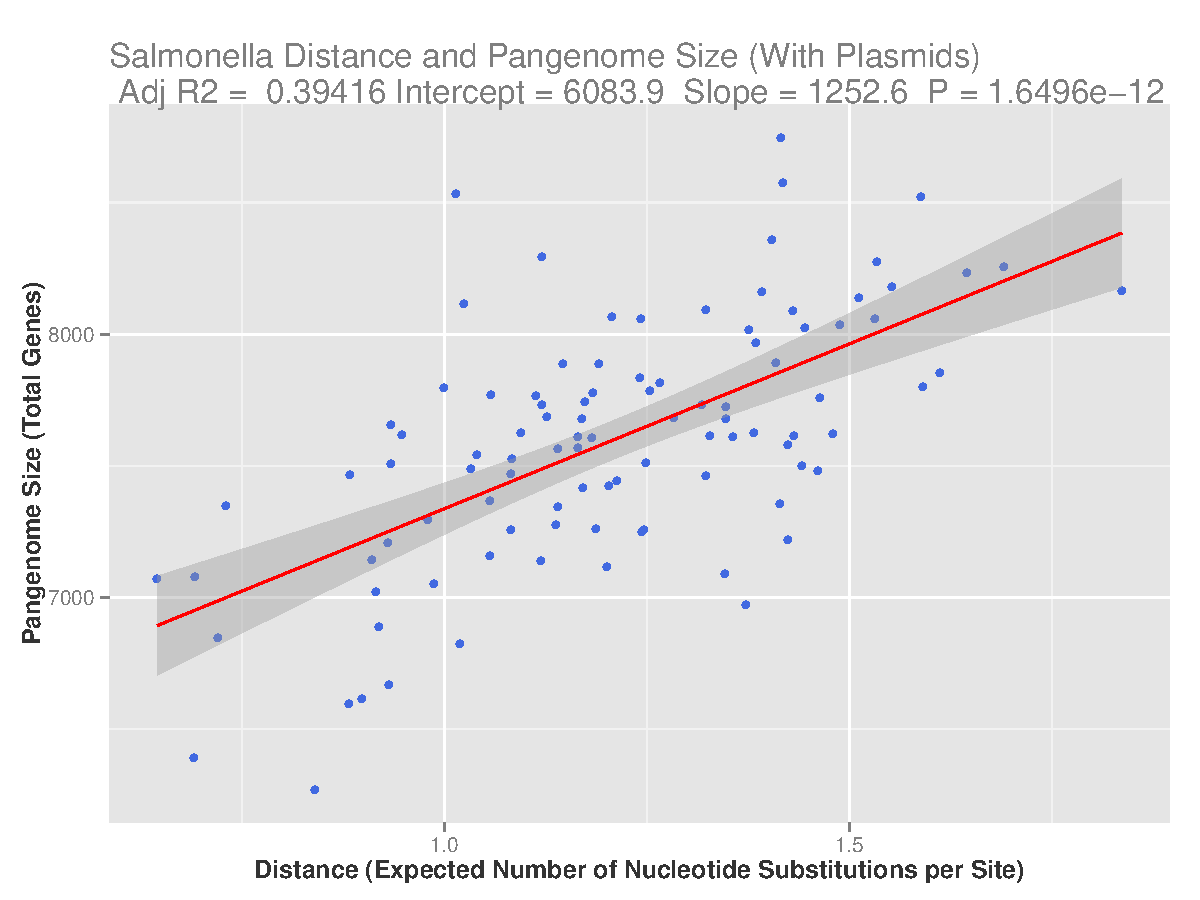
\includegraphics[width=\textwidth]{salmwithplasmidplots.pdf}

\begin{lstlisting}
Residuals:
    Min      1Q  Median      3Q     Max 
    -867.44 -248.82   34.71  208.10 1180.96 

Coefficients:
           Estimate Std. Error t value Pr(>|t|)    
Intercept)   6083.9      190.8  31.887  < 2e-16 ***
distance     1252.6      154.9   8.088 1.65e-12 ***
---
Signif. codes:  0  ***  0.001  **  0.01  *  0.05 . 0.1   1

Residual standard error: 369.3 on 98 degrees of freedom
Multiple R-squared:  0.4003,    Adjusted R-squared:  0.3942 
F-statistic: 65.41 on 1 and 98 DF,  p-value: 1.65e-12
\end{lstlisting}

\newpage

{\large \textbf{\salm}\\}
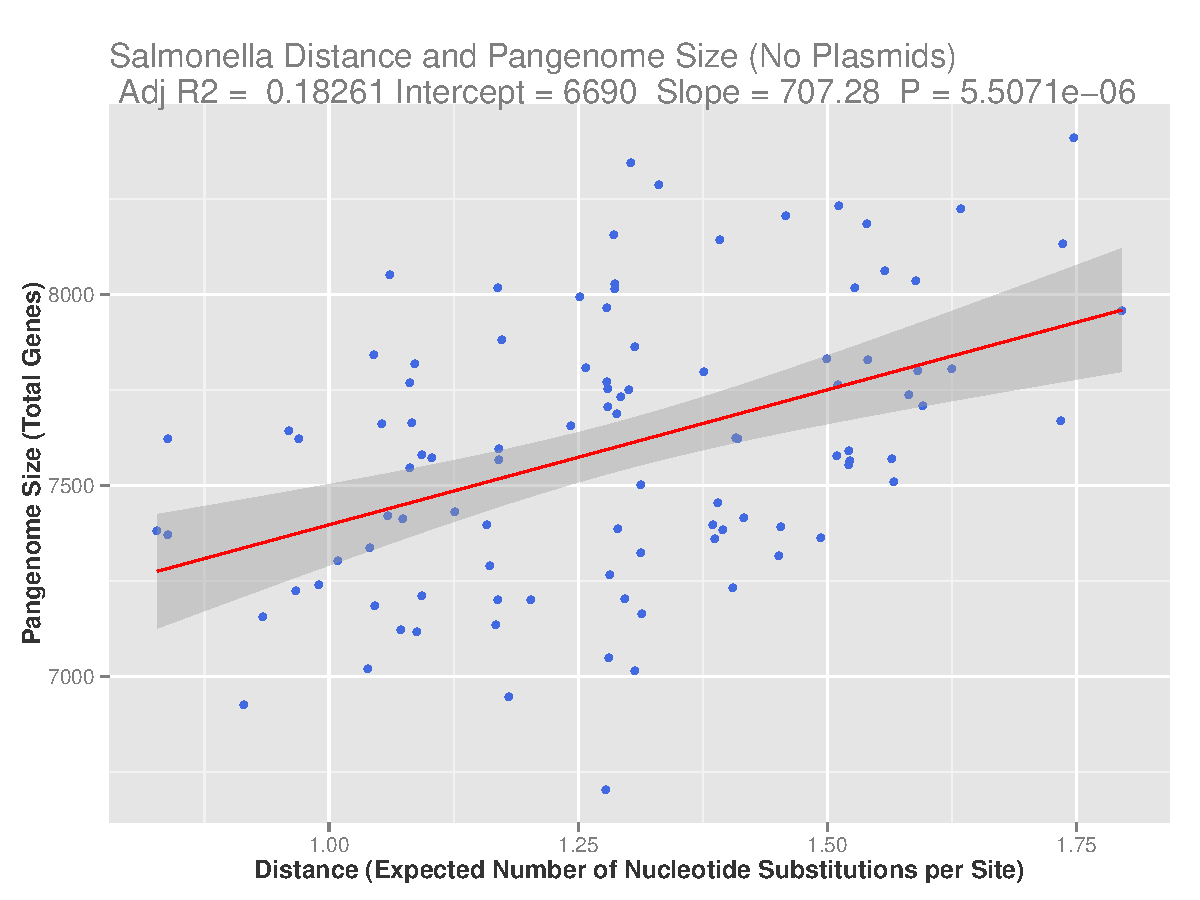
\includegraphics[width=\textwidth]{salmwoplasmidplot.pdf}

\begin{lstlisting}

Residuals:
    Min      1Q  Median      3Q     Max 
-890.36 -247.15  -16.13  232.67  733.39 

Coefficients:
            Estimate Std. Error t value Pr(>|t|)    
(Intercept)   6690.0      192.3  34.789  < 2e-16 ***
distance       707.3      147.1   4.808 5.51e-06 ***
---
Signif. codes:  0 *** 0.001 ** 0.01 * 0.05 . 0.1   1

Residual standard error: 323.1 on 98 degrees of freedom
Multiple R-squared:  0.1909,    Adjusted R-squared:  0.1826 
F-statistic: 23.12 on 1 and 98 DF,  p-value: 5.507e-06

\end{lstlisting}


\newpage 

{\large \textbf{\ecol}\\}
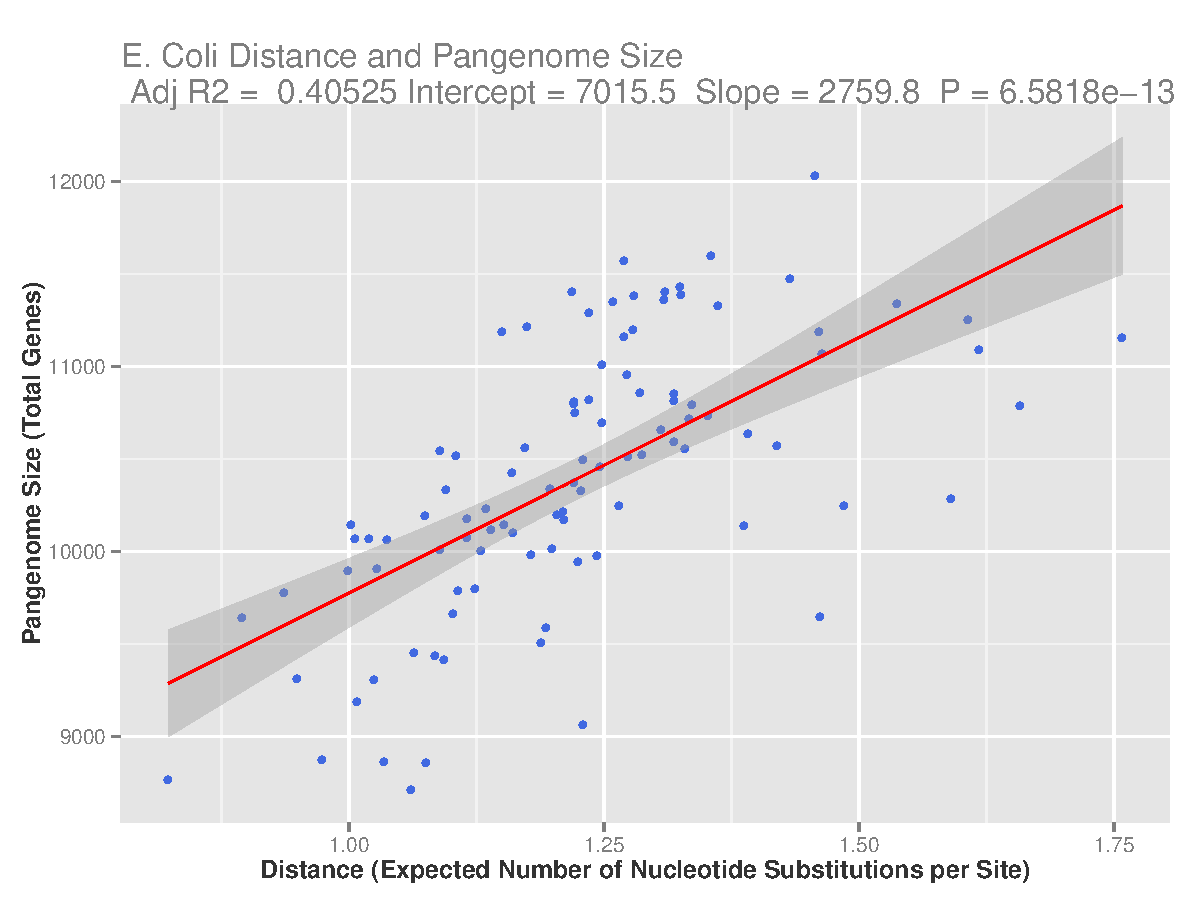
\includegraphics[width=\textwidth]{ecoliplotlr.pdf}

\begin{lstlisting}

Residuals:
     Min       1Q   Median       3Q      Max 
-1402.98  -320.12    16.56   360.71  1050.86 

Coefficients:
            Estimate Std. Error t value Pr(>|t|)    
(Intercept)   7015.5      412.7  16.997  < 2e-16 ***
distance      2759.8      333.6   8.274 6.58e-13 ***
---
Signif. codes:  0  ***  0.001  **  0.01  *  0.05  .  0.1     1

Residual standard error: 559.6 on 98 degrees of freedom
Multiple R-squared:  0.4113,    Adjusted R-squared:  0.4053 
F-statistic: 68.46 on 1 and 98 DF,  p-value: 6.582e-13

\end{lstlisting}

\newpage

{\large \textbf{\textit{L. monocytogenes}}\\}
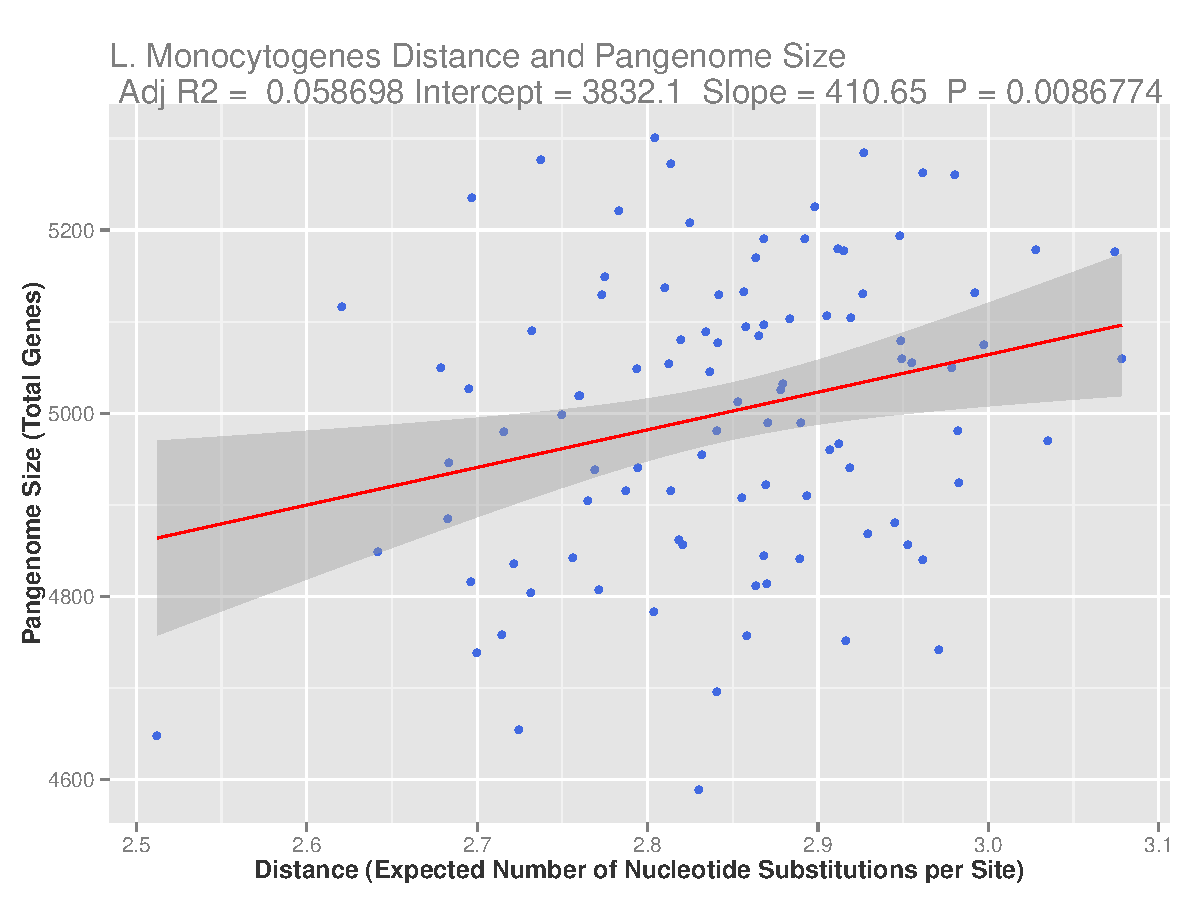
\includegraphics[width=\textwidth]{lmonoplotlr.pdf}

\begin{lstlisting}

Residuals:
    Min      1Q  Median      3Q     Max 
-405.30 -115.82   12.03   98.10  320.87 

Coefficients:
            Estimate Std. Error t value Pr(>|t|)    
(Intercept)   3832.1      436.6   8.777 5.42e-14 ***
distance       410.7      153.3   2.678  0.00868 ** 
---
Signif. codes:  0  ***  0.001  **  0.01  *  0.05  .  0.1     1

Residual standard error: 156 on 98 degrees of freedom
Multiple R-squared:  0.06821,   Adjusted R-squared:  0.0587 
F-statistic: 7.173 on 1 and 98 DF,  p-value: 0.008677


\end{lstlisting} 

\newpage

{\large \textbf{\textit{S.aureus}}\\}
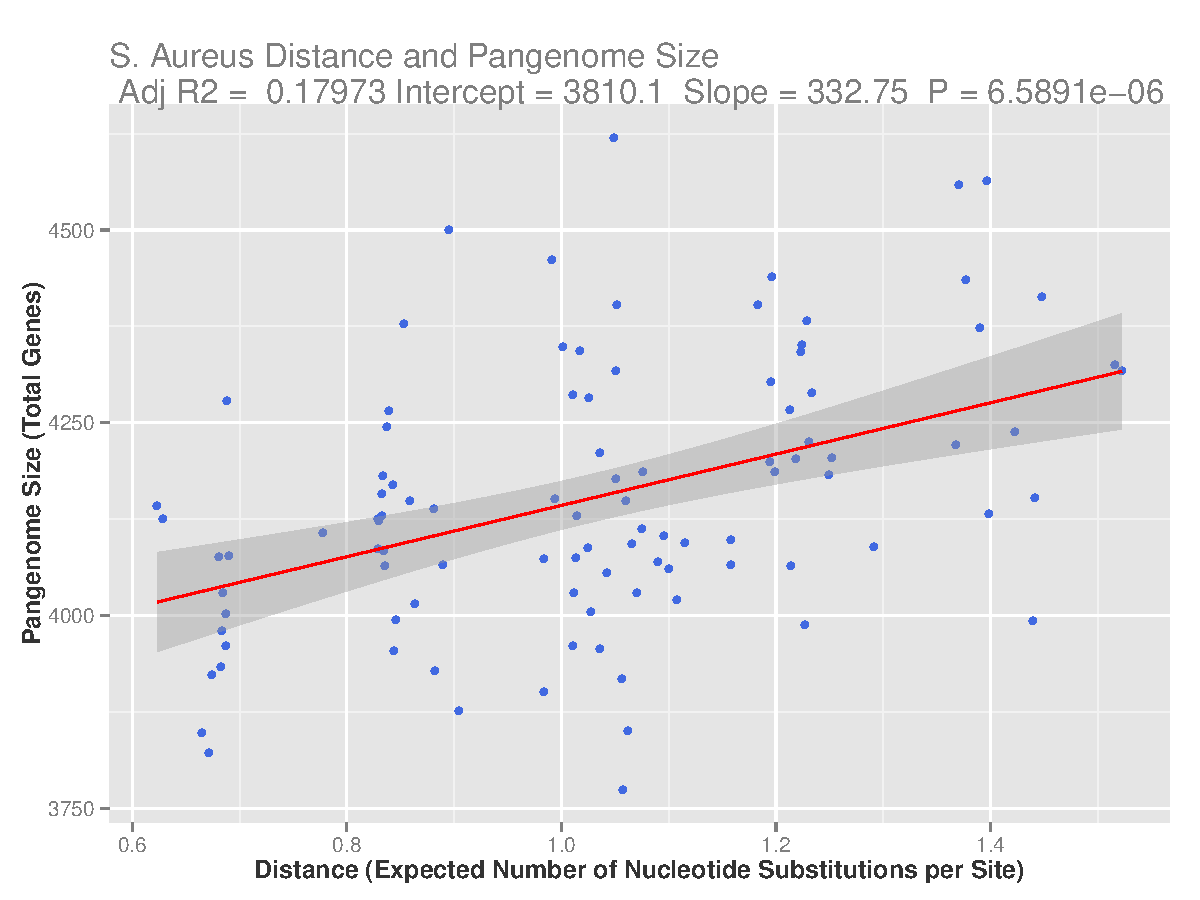
\includegraphics[width=\textwidth]{saureusplotlr.pdf}

\begin{lstlisting}

Residuals:
    Min      1Q  Median      3Q     Max 
-387.80 -102.91  -10.11   96.52  461.03 

Coefficients:
            Estimate Std. Error t value Pr(>|t|)    
(Intercept)  3810.05      73.66  51.723  < 2e-16 ***
distance      332.75      69.85   4.764 6.59e-06 ***
---
Signif. codes:  0  ***  0.001  **  0.01  *  0.05  .  0.1     1

Residual standard error: 156.5 on 98 degrees of freedom
Multiple R-squared:  0.188,     Adjusted R-squared:  0.1797 
F-statistic: 22.69 on 1 and 98 DF,  p-value: 6.589e-06
\end{lstlisting}

\newpage

{\large \textbf{\textit{S.pyogenes}}\\}
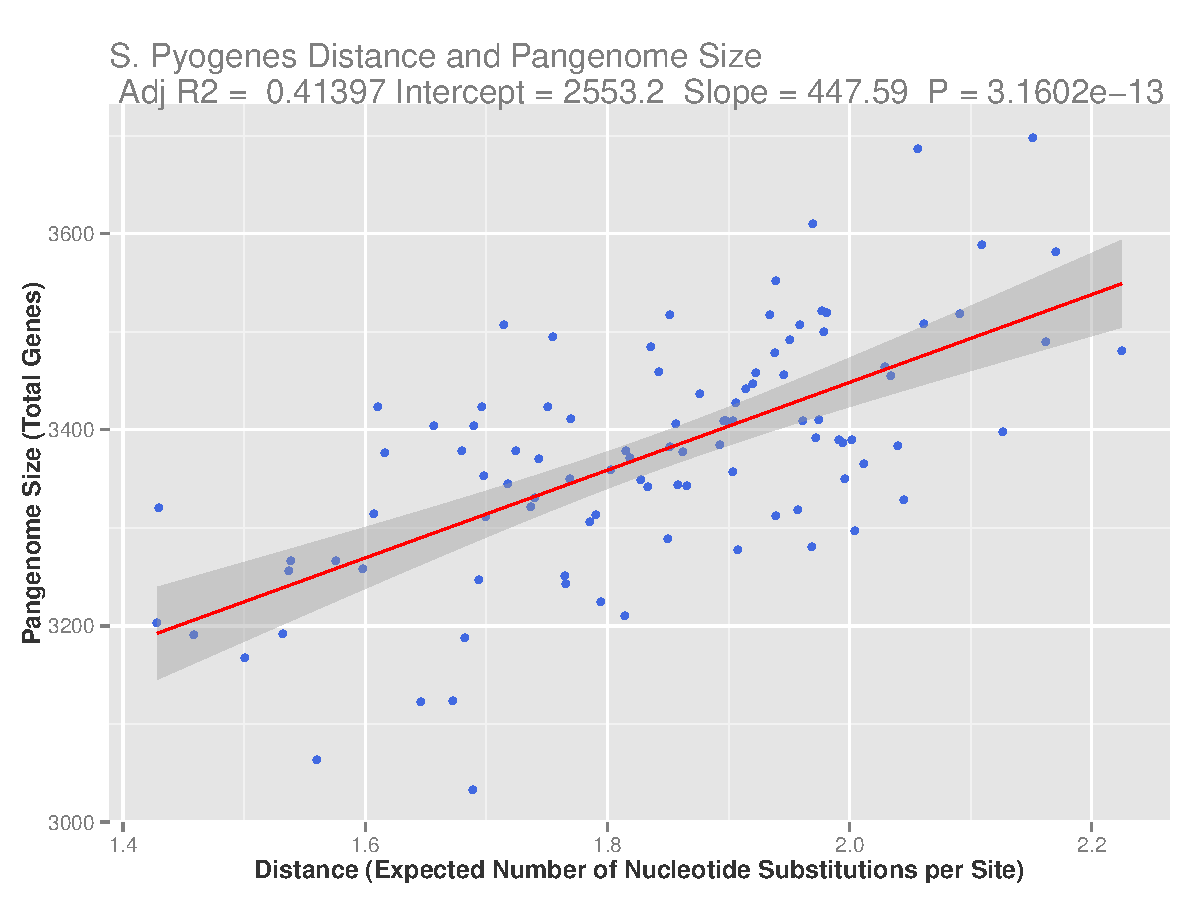
\includegraphics[width=\textwidth]{spyogenesplot.pdf}

\begin{lstlisting}

Residuals:
     Min       1Q   Median       3Q      Max 
-276.200  -55.087    4.264   58.879  213.287 

Coefficients:
            Estimate Std. Error t value Pr(>|t|)    
(Intercept)  2553.23      98.21  25.998  < 2e-16 ***
distance      447.59      53.14   8.422 3.16e-13 ***
---
Signif. codes:  0  ***  0.001  **  0.01  *  0.05  .  0.1     1

Residual standard error: 92.02 on 98 degrees of freedom
Multiple R-squared:  0.4199,    Adjusted R-squared:  0.414 
F-statistic: 70.93 on 1 and 98 DF,  p-value: 3.16e-13


\end{lstlisting} 

\newpage


{\large \textbf{\textit{C. jejuni}}\\}
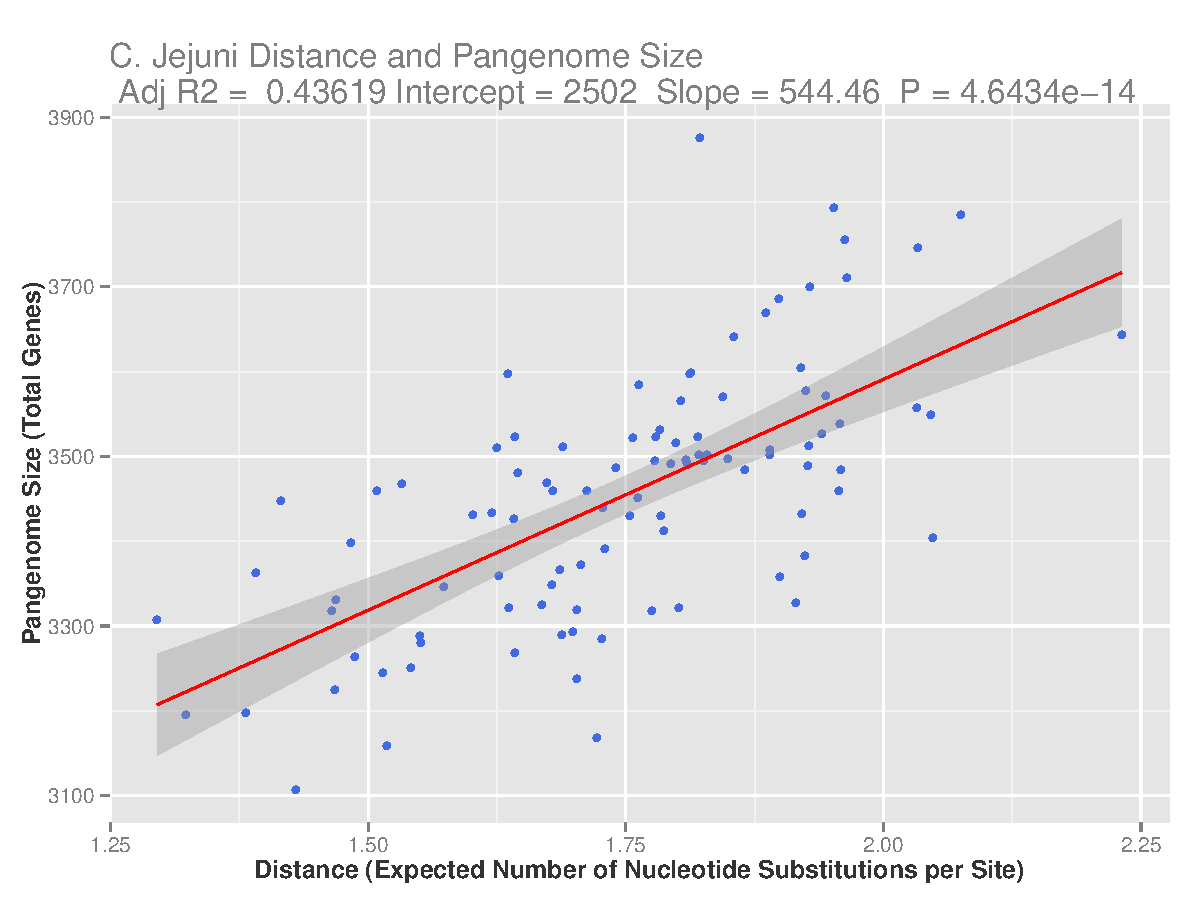
\includegraphics[width=\textwidth]{campyl_plot.pdf}

\begin{lstlisting}

Residuals:
    Min      1Q  Median      3Q     Max 
-271.35  -66.78   -2.52   68.55  382.06 

Coefficients:
            Estimate Std. Error t value Pr(>|t|)    
(Intercept)  2501.96     108.62  23.035  < 2e-16 ***
distance      544.46      61.81   8.809 4.64e-14 ***
---
Signif. codes:  0  ***  0.001  **  0.01  *  0.05  .  0.1     1

Residual standard error: 111.6 on 98 degrees of freedom
Multiple R-squared:  0.4419,    Adjusted R-squared:  0.4362 
F-statistic: 77.59 on 1 and 98 DF,  p-value: 4.643e-14

\end{lstlisting}

\newpage 

{\large \textbf{\textit{K. pneumoniae}}\\}
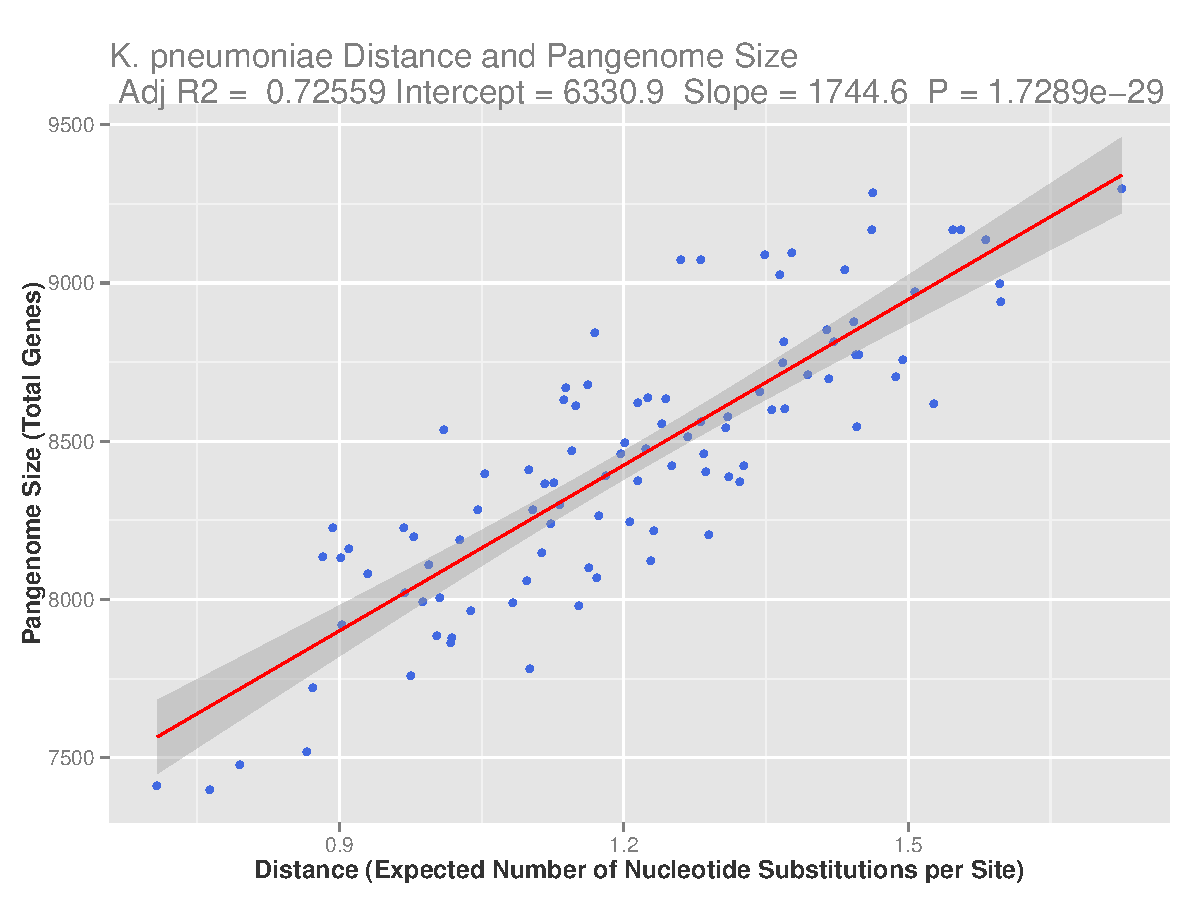
\includegraphics[width=\textwidth]{pneumoplot.pdf}

\begin{lstlisting}

Residuals:
    Min      1Q  Median      3Q     Max 
-470.28 -176.73   -3.73  138.30  543.38 

Coefficients:
            Estimate Std. Error t value Pr(>|t|)    
(Intercept)   6330.9      132.0   47.97   <2e-16 ***
distance      1744.6      107.6   16.21   <2e-16 ***
---
Signif. codes:  0  ***  0.001  **  0.01  *  0.05  .  0.1     1

Residual standard error: 223.6 on 98 degrees of freedom
Multiple R-squared:  0.7284,    Adjusted R-squared:  0.7256 
F-statistic: 262.8 on 1 and 98 DF,  p-value: < 2.2e-16


\end{lstlisting}

\newpage

{\large \textbf{\textit{Y. pestis (Roary with plasmids)}}\\}
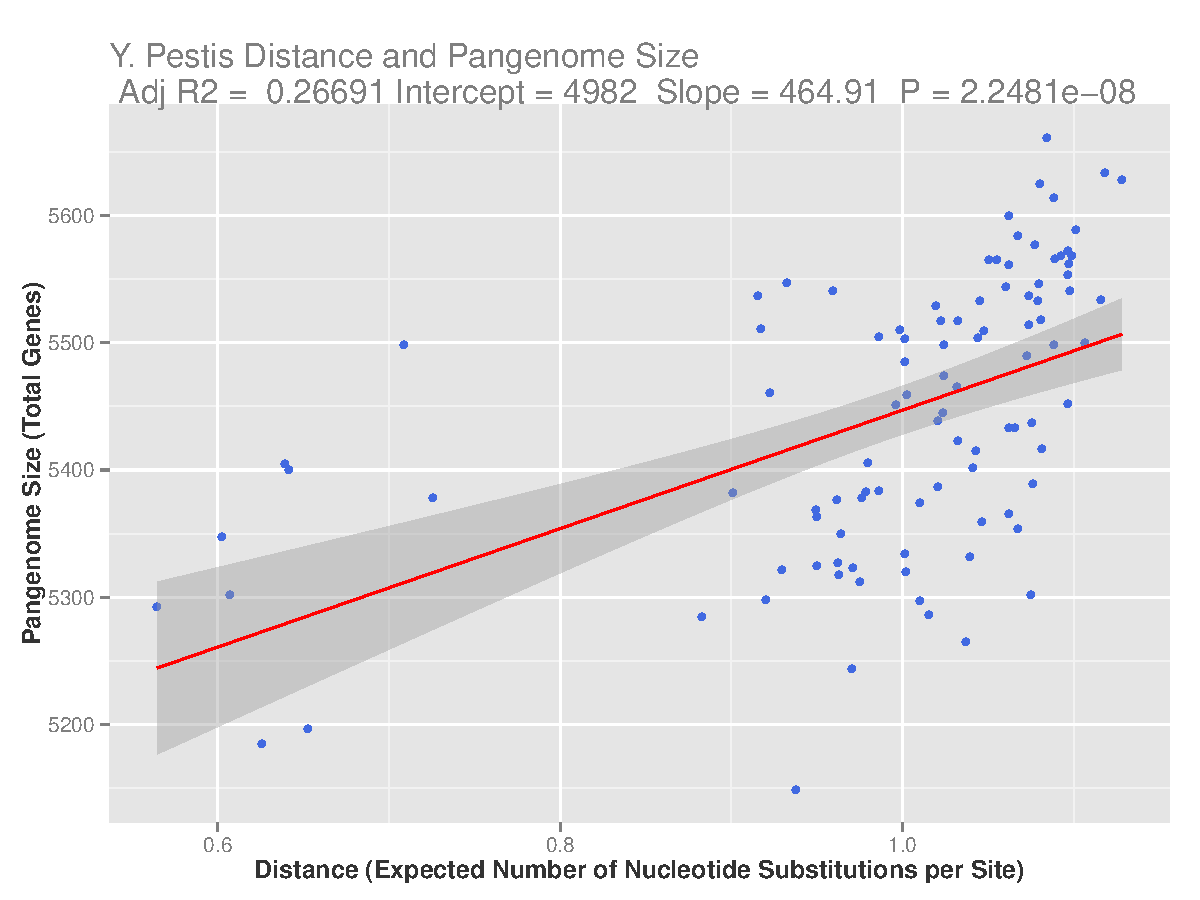
\includegraphics[width=\textwidth]{pestisplot.pdf}

\begin{lstlisting}
Residuals:
    Min      1Q  Median      3Q     Max 
-269.14  -71.55   13.31   70.56  186.45 

Coefficients:
            Estimate Std. Error t value Pr(>|t|)    
(Intercept)  4982.04      76.43  65.181  < 2e-16 ***
distance      464.91      76.38   6.087 2.25e-08 ***
---
Signif. codes:  0  ***  0.001  **  0.01  *  0.05  .  0.1     1

Residual standard error: 95.16 on 98 degrees of freedom
Multiple R-squared:  0.2743,    Adjusted R-squared:  0.2669 
F-statistic: 37.05 on 1 and 98 DF,  p-value: 2.248e-08
\end{lstlisting}

\newpage

{\large \textbf{\textit{Y. Pestis (no plasmids)}}\\}
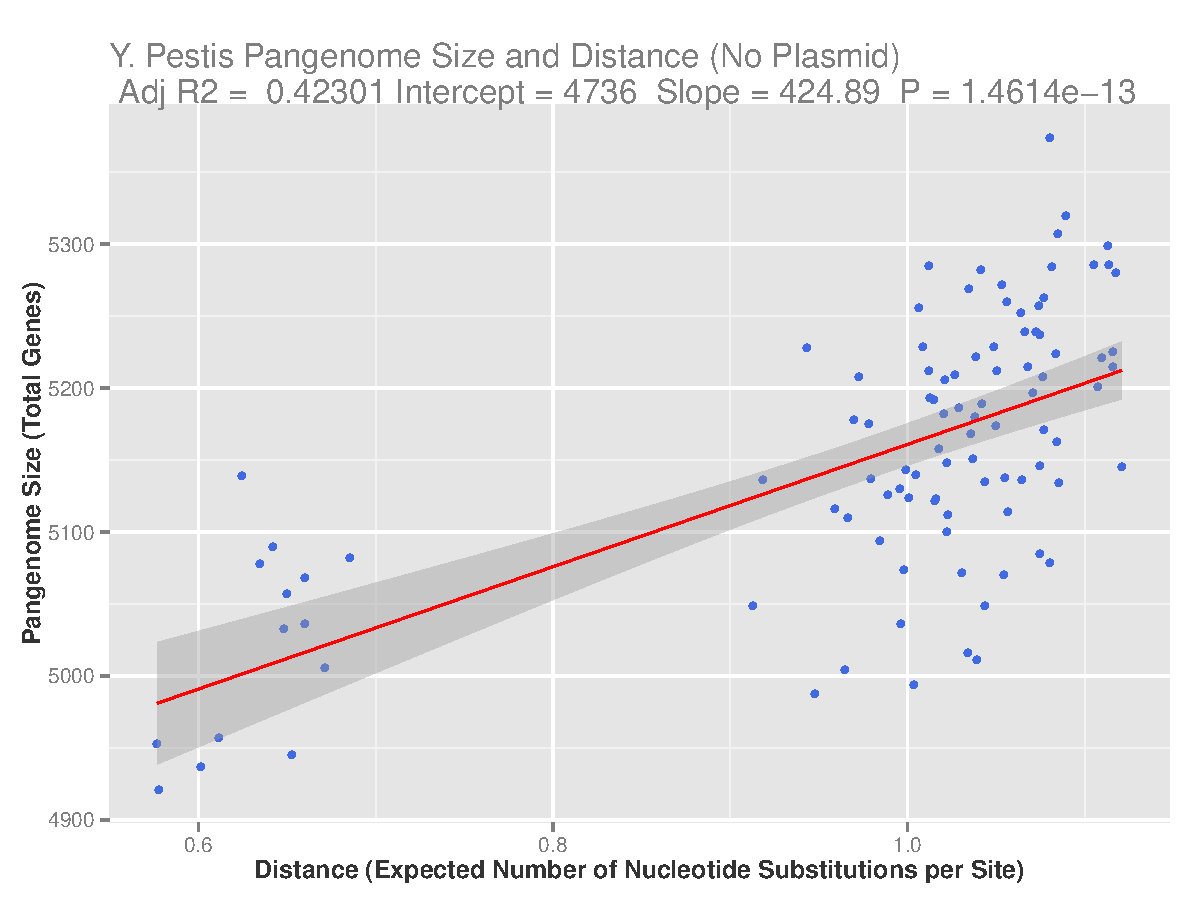
\includegraphics[width=\textwidth]{ypestnoplasmplot.pdf}


\begin{lstlisting}

Residuals:
     Min       1Q   Median       3Q      Max 
-168.458  -45.574    8.002   50.453  178.932 

Coefficients:
            Estimate Std. Error t value Pr(>|t|)    
(Intercept)  4735.96      49.17  96.326  < 2e-16 ***
distance      424.89      49.53   8.578 1.46e-13 ***
---
Signif. codes:  0  ***  0.001  **  0.01  *  0.05  .  0.1     1

Residual standard error: 72.68 on 98 degrees of freedom
Multiple R-squared:  0.4288,    Adjusted R-squared:  0.423 
F-statistic: 73.58 on 1 and 98 DF,  p-value: 1.461e-13


\end{lstlisting}

\newpage

{\large \textbf{\textit{H. pylori}}\\}
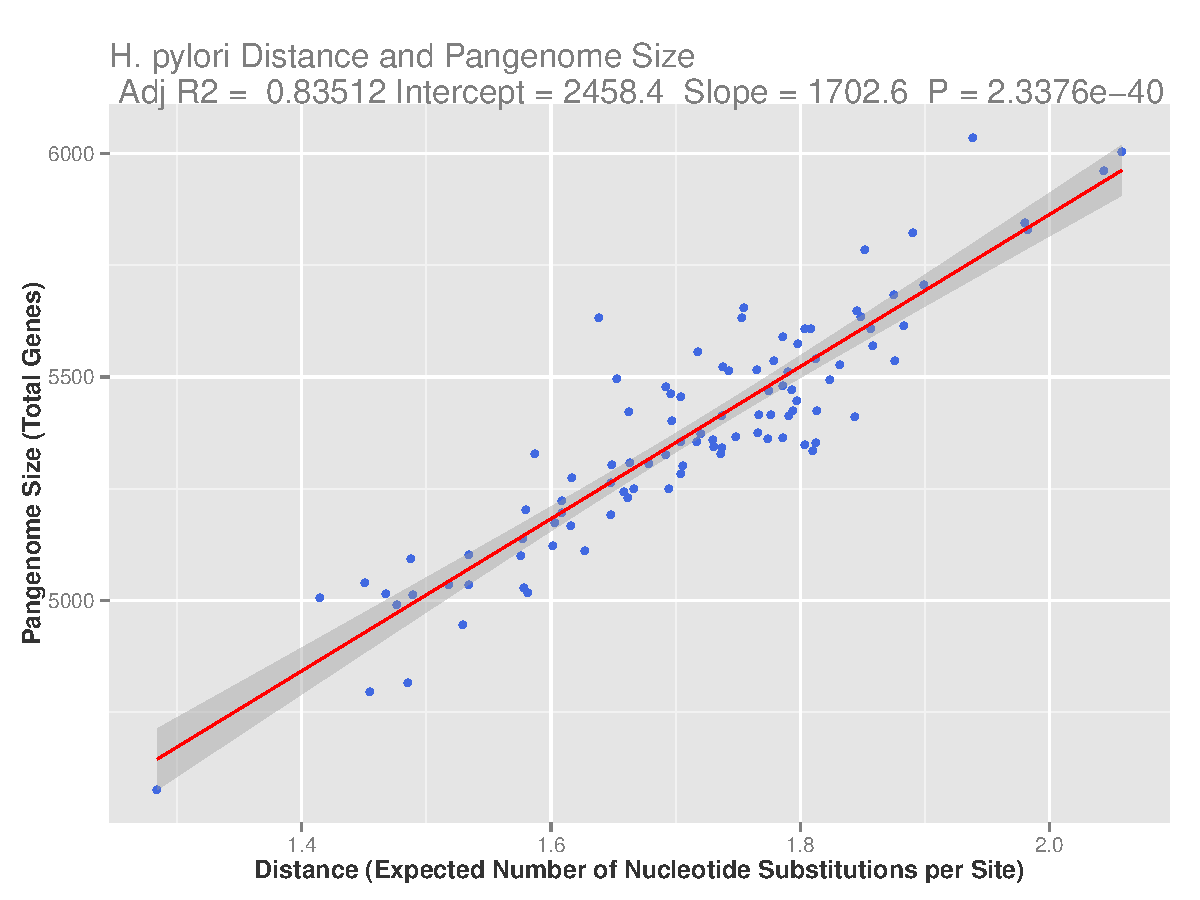
\includegraphics[width=\textwidth]{hpyloriplot.pdf}

\begin{lstlisting}

Residuals:
    Min      1Q  Median      3Q     Max 
-204.67  -68.46   -9.40   54.63  385.49 

Coefficients:
            Estimate Std. Error t value Pr(>|t|)    
(Intercept)  2458.40     130.57   18.83   <2e-16 ***
distance     1702.57      75.96   22.41   <2e-16 ***
---
Signif. codes:  0  ***  0.001  **  0.01  *  0.05  .  0.1   1

Residual standard error: 104.6 on 98 degrees of freedom
Multiple R-squared:  0.8368,    Adjusted R-squared:  0.8351 
F-statistic: 502.4 on 1 and 98 DF,  p-value: < 2.2e-16

\end{lstlisting}


{\large \textbf{\textit{M. tuberculosis}}\\}
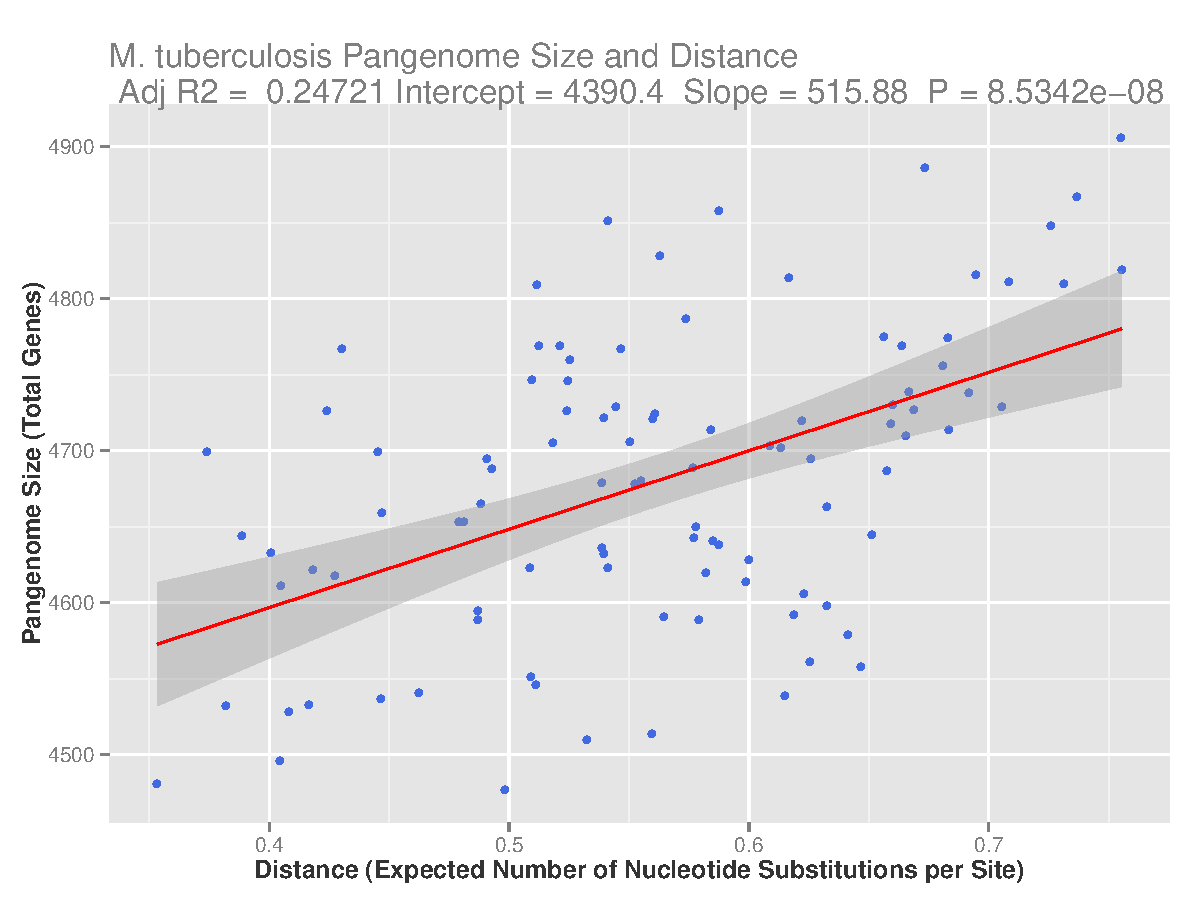
\includegraphics[width=\textwidth]{tuber_plot.pdf}

\begin{lstlisting}

Residuals:
    Min      1Q  Median      3Q     Max 
-269.14  -71.55   13.31   70.56  186.45 

Coefficients:
            Estimate Std. Error t value Pr(>|t|)    
(Intercept)  4982.04      76.43  65.181  < 2e-16 ***
distance      464.91      76.38   6.087 2.25e-08 ***
---
Signif. codes:  0  ***  0.001  **  0.01  *  0.05  .  0.1   1

Residual standard error: 95.16 on 98 degrees of freedom
Multiple R-squared:  0.2743,    Adjusted R-squared:  0.2669 
F-statistic: 37.05 on 1 and 98 DF,  p-value: 2.248e-08

\end{lstlisting}



\end{document}
